% !TeX root = ../main.tex
% Add the above to each chapter to make compiling the PDF easier in some editors.

\chapter{Funboy, the DARVAH Implementation}\label{chapter:implementation}

In this chapter, we will provide the implementation details. Funboy is the module that offers the DARVAH loop functionality inside of the Ravestate Dialogue System. This approach allowed us to seamlessly integrate the current dialogue functionality with the new capabilities which we developed to conduct the experiment (see Chapter~\ref{chapter:experiment}). Figure \ref{fig:system} illustrates the full system overview.

There are several components in the system:
\begin{itemize}
    \item Funboy is a Ravestate module that implements the main loop of the DARVAH framework. 
    \item GPT-2 TLH is a GPT-2-based \acrshort{dnn} Language Model conditioned on humour data via Transfer Learning.
    \item Funboyn4j is a Docker container that provides persistence for users' humour profiles via Neo4j graph database instance running inside of the container.
    \item Rosemo is an emotion recognition software that contains EmoPy \acrlong{fer} and \acrfull{ser} software modules to support processing and evaluating emotions. We deploy Rosemo in a Docker container as well.
    \item Roboy Sonosco for speech synthesis and roboy\_speech\_recognition for speech recognition capabilities. Both packages use Google Speech Services to provide functionality.
    \item The interfaces between the parts use ROS 1.0 and web-sockets for communication.
\end{itemize}

\begin{figure}[htpb]
  \centering
  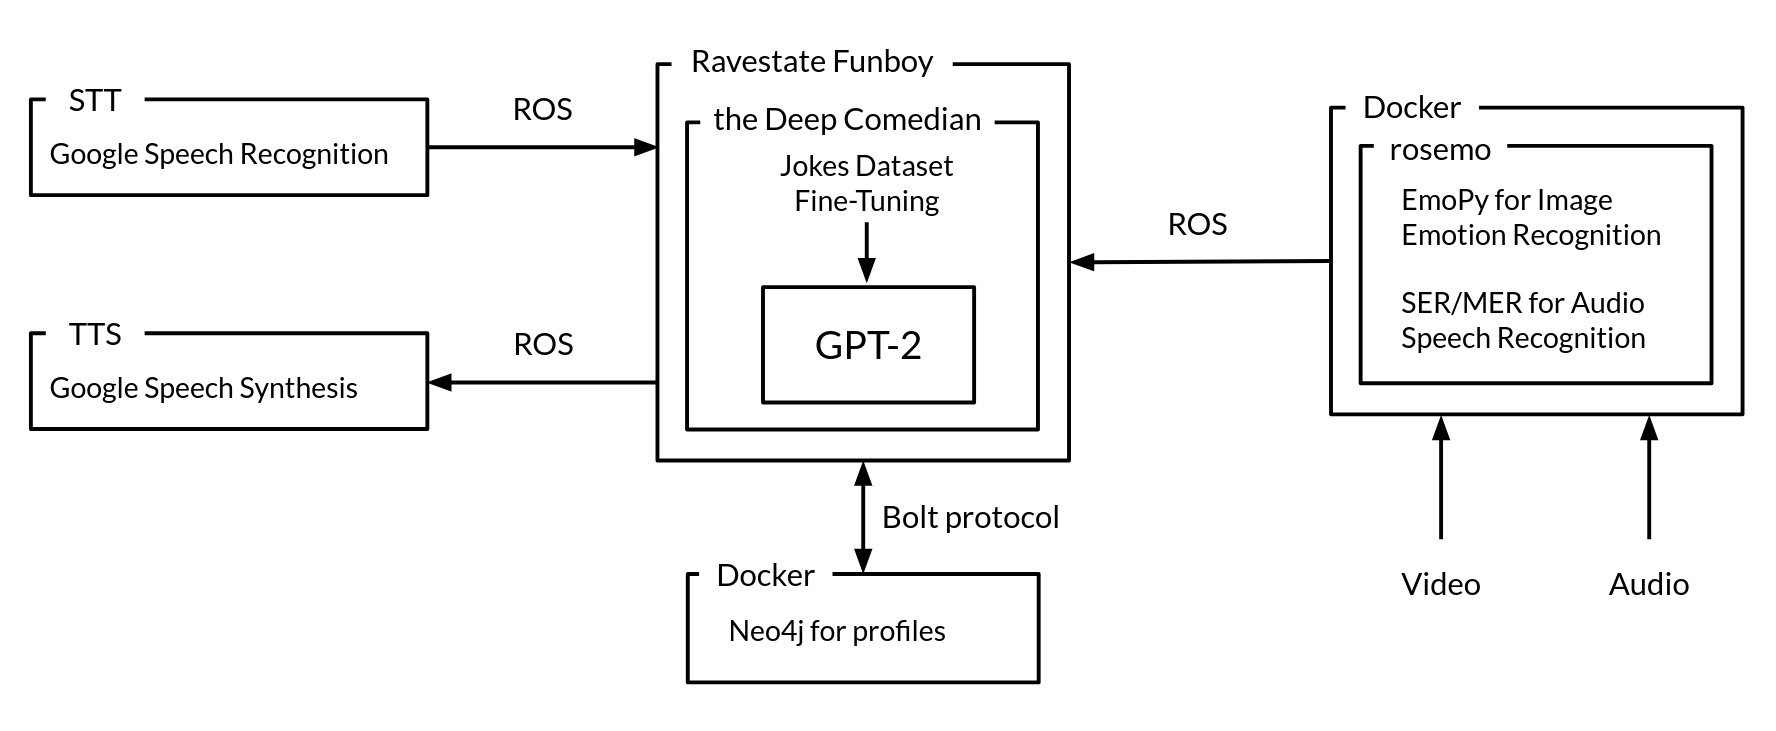
\includegraphics[width=1.0\textwidth]{figures/system.png}
  \caption{The system implementing Funboy - DARVAH for Roboy.} \label{fig:system}
\end{figure}

The system employs the following important dependencies used in development and deployment and is guaranteed to work with the stated versions of the software distributions:
\begin{itemize}
    \item Python 3.6 is the target Python version\footnote{by default we assume this version anywhere we mention Python} for Ravestate
    \item Docker 19.03 to deploy the containers
    \item Rosemo with EmoPy (version from 23.01.2020 on GitHub) and \acrshort{ser} (version from 28.06.2019 on GitHub)
    \item ROS 1.0 Kinetic or Melodic for ROS-based interfaces on Ubuntu 16.04 or 18.04 respectively 
    \item roboy\_communication package containing all ROS messages and nodes for Roboy
    \item Tensorflow 1.15.2 for EmoPy and \acrshort{ser} to run the models on CPU
    \item Tensorflow-gpu 1.15.2 to run GPT-2 TLH on GPU
    \item CUDA 10.0 and CuDNN 7.6.4 for GPU computing capabilities
    \item ScientIO 0.9.0 to interface from Ravestate to Neo4j
    \item neo4j-driver 1.7.6 to provide a Neo4j database driver for ScientIO
    \item Neo4j 3.5 for compatibility with neo4j-driver
    \item PyAudio 0.2.11 for audio processing capabilities
\end{itemize}
It is important to note that even if the full implementation does not need an embodied robot to work, it is not fully independent from Roboy as it heavily uses software distributed by the Roboy project. However, all Roboy-developed software adheres to open-source principles and follows permissive licensing practices.

\section{Ravestate Funboy Module}

Funboy is a proof-of-concept implementation of the DARVAH framework which we developed as a Ravestate module. Ravestate is not only the default Dialogue System for Roboy it also offers the system of abstractions very convenient for implementing the DARVAH loop in code (see Section~\ref{section:dialogues} in Chapter~\ref{chapter:background}).

We define all of the main Funboy module structures in the init file. It comprises six Ravestate states. The first state \( start()\) initialises the following Funboy Ravestate properties:
\begin{itemize}
    \item prop\_start\_time = rs.Property(name="start\_time"), the property defines a timestamp used to postpone start-up of the DARVAH deducing state \( D\).
    \item prop\_comedian = rs.Property(name="comedian"), the property defines the ComedianStrategy object.
    \item prop\_emotion = rs.Property(name="emotion"), the property defines the EmotionStrategy object.
\end{itemize}
The state activates on the condition rs.sig\_startup which occurs when the Ravestate starts up. 

The following state \( deduce()\) implements DARVAH's \( D\) functionality. It activates every time the Ravestate input triples change in the ravestate\_nlp module: nlp.prop\_triples.changed(). This state reads prop\_start\_time property and checks if it satisfies the \(\delta\) time constraint - if the difference between the current system time and the property is bigger than the constraint, it starts the DARVAH loop. Otherwise, other Ravestate dialogue states take precedence. If the DARVAH deducing process is successful, the state emits sig\_tell\_joke signal.

The third state is \(assess()\). Its activation condition is those mentioned above sig\_tell\_joke Ravestate signal. The state reads the interloc.prop\_all property which contains all the interlocutor's data in Ravestate. This property is necessary to access the affinity scores for joke types. When \(assess()\) selects the joke category, it writes the chosen category into prop\_joke\_category property.

The fourth \(render()\) state activates given two conditions: the sig\_tell\_joke and the prop\_joke\_category.changed() signals. Thus, after \(deduce()\) emits the signal, this state still waits for the \(assess()\) state to write into the prop\_joke\_category property. When both signals are present, the state accesses the ComedianStrategy object from the prop\_comedian property (see Subsection~\ref{subsection:comstr}). If necessary, it configures the strategy and calls the \(render()\) method. Based on the current utterance and chosen joke category, the state either skips the utterance to perform proactive humour generation or passes the utterance to perform reactive humour generation. Afterwards, the state emits the sig\_joke\_told signal.

The next state is \( validate()\) which activates given the sig\_joke\_told signal. This state reads the EmotionStrategy object prop\_emotion property (see Subsection~\ref{subsection:emostr}). If necessary, it configures the strategy and calls its \(get\_positivity()\) method. Then, \( validate()\) evaluates the received values and writes the evaluation result into prop\_emotion\_val.

The last one is the \(attune()\) state. It activates when two conditions are present: the sig\_tell\_joke and the prop\_emotion\_val.changed() signals. The state reads the prop\_joke\_category and the interloc.prop\_all properties to access the affinity scores of the current interlocutor. Based on the validation result, it changes the score of the joke type accordingly and writes back into interloc.prop\_all. When the writing process is done, \(attune()\) emits sig\_joke\_finish to restart the Funboy's DARVAH loop.

\subsection{ComedianStrategy}\label{subsection:comstr}

\begin{figure}[htpb]
  \centering
  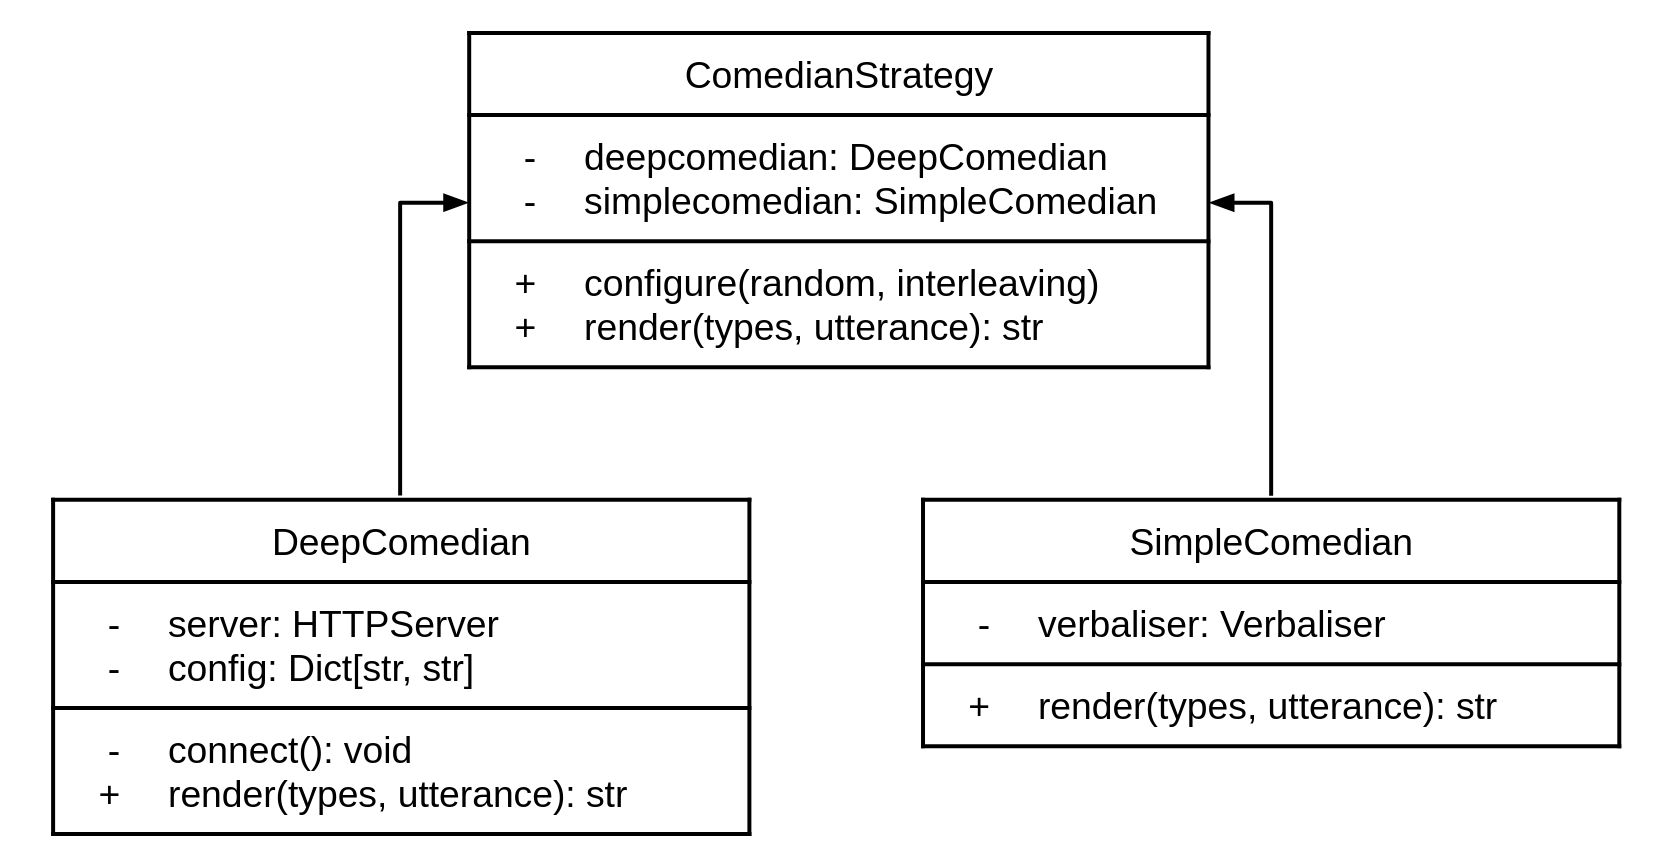
\includegraphics[width=0.8\textwidth]{figures/umlcomstr.png}
  \caption{The UML diagram for ComedianStartegy.} \label{fig:umlcs}
\end{figure}

ComedianStrategy is a class that implements the strategy pattern for the joke generation process (see the listing for this class in Appendix~\ref{appendix:comedian}). When initialised, it creates both DeepComedian and SimpleComedian objects (see Figure~\ref{fig:umlcs} and Section~\ref{section:deepc}). The constructor accepts one parameter, which is the threshold value for the Random strategy's random number generator (default value is 0.5).

The class features a simple interface that offers two methods:
\begin{itemize}
    \item configure(self, random: bool = False, interleaving: bool = False) - this method defines the current strategy. There are three available strategies:
    \begin{enumerate}
        \item Interleaving strategy - this strategy chooses either SimpleComedian for even calls or DeepComedian alternately for odd calls.
        \item Random strategy - this strategy randomly selects either DeepComedian or SimpleComedian according to the defined probability threshold.
        \item Default strategy - this strategy selects only DeepComedian.
    \end{enumerate}
    \item render(self, type, utterance: str) -> str - this method provides the interface to the Comedian render() method with the same signature. When called, it calls this method of either DeepComedian or SimpleComedian and returns the generated string.
\end{itemize}

\section{DeepComedian and SimpleComedian}\label{section:deepc}
Includes the DeepComedian and the SimpleComedian as implementations of the DARVAH's Comedian sub-component.

\begin{figure}[htpb]
  \centering
  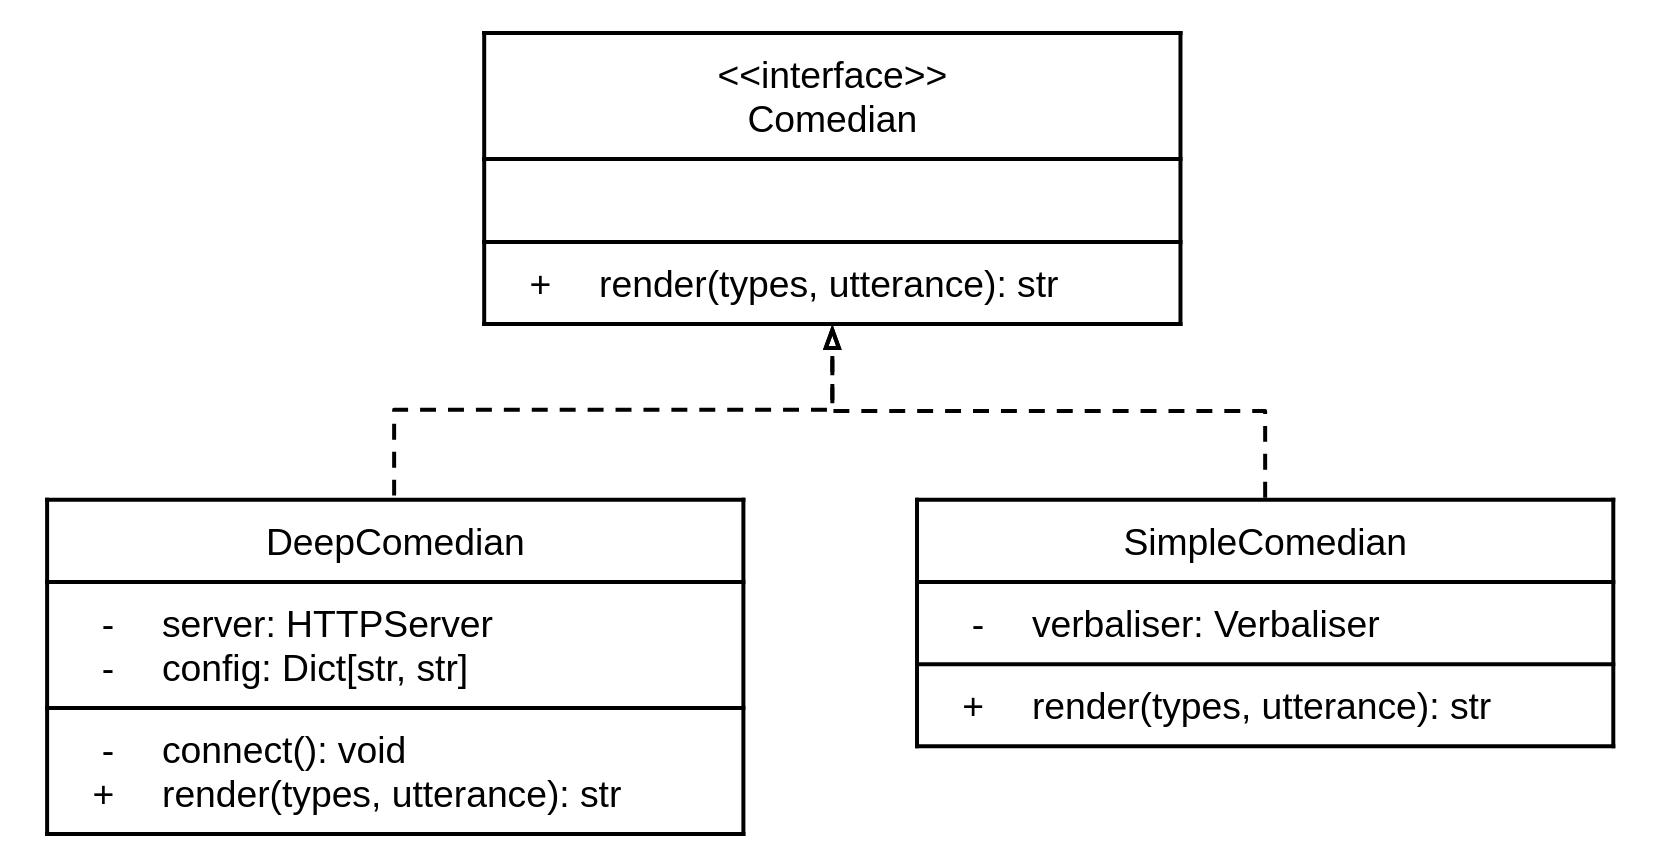
\includegraphics[width=0.8\textwidth]{figures/umlcomed.png}
  \caption{The UML diagram for Comedian classes.} \label{fig:umlci}
\end{figure}

\subsection{Language Model}
As a baseline Language Model for the rendering state \( R\), we have selected the 744-million-parameters GPT-2-L model~\parencite{gpt2}. The model is the second biggest one of all currently available GPT-2 models, which is beneficial for solving Natural Language Generation problems because more parameters yield better quality. At the same time, the biggest model, GPT-2-XL, offers only a minor increase in \acrshort{nlg} quality while being too large to run locally on our hardware~\parencite{radford2019language}.

To test how well the GPT-2-L model generates text, we provided an initial prompt for completion denoted by IP. 
\begin{itemize}
    \item IP:    Why are robots shy? 
\end{itemize}

The model generated following completions (here, we selected shorter clauses from all generated samples):
\begin{itemize}
    \item A1:    The answer is likely a combination of genetics and programming. 
    \item A2:    They are not shy because they are not human.
    \item A3:    Robots don't like getting too close to people or touching people.
    \item A4:    It's hard to say for sure.
    \item A5:    Because it takes a lot to get one's attention.
    \item A6:    It's not what they're afraid of but what you're afraid of.
\end{itemize}

All clauses form comprehensible phrases (excluded ones as well). However, their humorous effect is low when compared to a human-generated answer HA:
\begin{itemize}
    \item HA:    Because they have hardware and software but no underwear.
\end{itemize}    

To overcome this drawback, we decided to modify the model via transfer learning.

\subsection{Transfer Learning}
Transfer learning is a concept which allows applying previously learned knowledge from one domain or problem to another domain or problem. The process is similar to how humans can leverage their mental models based on ideas which they learned before~\parencite{transferlearn}. However, unlike humans, Roboy cannot do it automatically and requires us to adjust the model.

We could instead train the GPT-2-L from scratch using our dataset of jokes. Usually, in our case, it is impractical because the GPT-2-L features a substantial size. It is a Deep Model comprising 774 million parameters trained on a dataset of 8 million webpages (40 GB of plain text)~\parencite{radford2019language}. Thus, the model’s size poses a challenge to the data collection and makes it infeasible to train by us because of the extreme computational requirements. However, transfer learning helps us to solve this issue by utilising already trained parameters’ values.

Transfer learning alleviates Deep Learning issues in three ways: lower data requirements, smaller memory and processing requirements, shorter training time. For example, training a full GPT-2-L might take several weeks while the transfer learning allows having a new model in under a day depending on the size of the dataset~\parencite{transferlearn}.

To adapt the model for transfer learning, we could follow either of two approaches. The first one is to keep the pre-trained model architecture and weights. This way, we need to add several new layers at the output of the original model, or we can use the model output as input to a new smaller model. This approach is suitable if the target problem stays the same.

Another method is to modify the internal architecture of the original. The approach is useful if we want to adapt to a different target problem in the same domain. In this case, we could have used the pre-trained model to initialise a new model, including problem-specific changes such as adding skip or residual connections or using bottleneck modules between the layers of the original model.

However, in our case, the optimal choice was to adhere to the former approach due to two reasons. Firstly, the domain stays similar because the GPT-2-L provides the English language model while we would like to have the English humour (language) model, which narrows down the original domain to more specific textual representations. Secondly, the size of the GPT-2-L architecture makes it unfeasible to pursue the second approach due to time and computational constraints. Finally, the target task remains the same - generation of natural language sentences.

To perform transfer learning using GPT-2-L, we update Transformer layers (see Figure \ref{fig:gpt}) with the encoded joke data using original GPT-2 model and encoder from its GitHub repository \parencite{gpt2}.

\subsection{Roboy Jokes Dataset}

To assemble the dataset, we decided to employ online data sources since there is not much ready-to-use joke data available publicly. For most of our data, we used the Pushift project~\parencite{baumgartner2020pushshift} to access cached data from Reddit forums (subreddits). The collected data consists of text posts from the following subreddits from the original date of the forum creation until 01.01.2020:
\begin{itemize}
    \item "jokes",
    \item "darkjokes",
    \item "dadjokes",
    \item "cleanjokes",
    \item "oneliners",
    \item "badjokes",
    \item "dirtyjokes",
    \item "DarkJokeCentral"
\end{itemize}
After we downloaded the data, we stripped it from all functional characters, removed empty and deleted samples, removed the jokes with offensive words or nonsensical data and chose their class labels. We also added data from the publicly available joke-dataset~\parencite{pungas} containing 208000 jokes from www.reddit.com, www.stupidstuff.org, www.wocka.com. All of the collected raw data contained over 1350000 data points. The resulting clean dataset contains over 800000 jokes.

Each line in the dataset is a separate joke. We annotated each line with an <|endofline|> label at the end of the line, to delimit where the previous joke ends and a new one starts. At the beginning of each line, we appended multiple class labels according to the following idea.

First, we split the jokes into groups according to their sizes. The introduced size classes are: 
\begin{itemize}
    \item "short" for lines of length smaller or equal to 200 characters.
    \item "medium" for lines of length bigger than 200 and smaller or equal to 400 characters.
    \item "long" for lines of length bigger than 400 and smaller or equal to 800 characters.
    \item "story" for lines of length bigger than 800 and smaller or equal to 1600 characters.
\end{itemize}
The choices of the lengths for the classes were based on the time it takes to pronounce the spoken utterances.

Besides the size classes, we split the dataset into 20 content classes based on token frequency. For example, we defined class \( c_1\)=<|c\_1|> through the token "chicken" and assigned the class to all samples for which the frequency of the token "chicken" was higher than other tokens' frequencies. The whole list of the class token contains 20 words: "chicken", "momma", "trump", "pet", "army", "police", "religion", "bar", "clown", "german", "date", "queer", "boss", "doctor", "british", "cookie", "family", "friend", "dadjokes", "other".
All classes that did not have a suitable token were assigned the token "other" for \( c_{20}\)=<|c\_20|>. However, during the initial joke generation testing, we realised that this approach introduced two disadvantages. First, many generated jokes were very close to the original data, which indicated that that the model was overfitting. Although, in our case, overfitting is not an entirely negative phenomenon since it is, for example, similar in nature to people reading and retelling jokes from elsewhere to their friends. However, we still wanted the model to produce more creative results.

The second disadvantage is that the set of classes was not extendable after the training process was finished. Usually, this is not a problem. For example, with the size classes, they can change only globally on the whole dataset. Thus we will need to retrain the model. However, let's consider the following situation.

We would like to generate a reactive response and we receive the following input utterance:
\begin{itemize}
    \item \( U_{t-1}^i = \)"Why are robots shy?"
\end{itemize}
For example, we selected \( l_1\)=<|l\_1|> size class. However, it is unclear which class we have to select from the content classes because, for the utterance \( U_{t-1}^i\):
\[ Subject(U_{t-1}^i)="robots"\]
which is not in the list of class tokens, thus the only viable choice would be to use token "other" and the associated class \( c_{20}\)=<|c\_20|>. We tried generating a response and obtained the following result:
\begin{itemize}
    \item Input prompt: "<|l\_1|> <|c\_20|>Why are robots shy?"
    \item \( U_{t}^r = \)"They have lower case letters than police."
\end{itemize}
which is semantically ambiguous.

Therefore we decided to switch to plain-text class labels. We reasoned that if the model can connect the label with the words in the joke string, we might be able to add more classes at runtime if needed. We replaced all labels according to their class token as in:
\begin{itemize}
    \item \(l_1\)=<|l\_1|> \(\rightarrow\) \(l_1\)=<|short|>
    \item \( c_1\)=<|c\_1|> \(\rightarrow\) \( c_1\)=<|chicken|>
\end{itemize}
Afterwards, we retrained our model and tested the same example with the new class labelling schema. At runtime, we generated a new class label \( c_{21}\)=<|\(Subject(U_{t-1}^i)\)|>=<|robots|> and tried generating a reactive response. We obtained the following result:
\begin{itemize}
    \item Input prompt: "<|short|> <|robots|>Why are robots shy?"
    \item \( U_{t}^r = \)"The only job robot does well is driving a bus."
\end{itemize}
which greatly improved semantically.

The change also slightly reduced overfitting of smaller jokes due to less restrictive labelling since the class labels are not unique strings.

\subsection{Training Process and Resulting Model}

We used download\_model.py script from OpenAI GPT-2 GitHub repository~\parencite{gpt2} to obtain their original pre-trained GPT-2 774M model. Although OpenAI originally trained the model using Tensorflow 1.12.0, it is fully compatible with Tensorflow 1.15.2 which we used for training. The model's checkpoint is over 3 GB in size and uses a Tensforflow 1.0 checkpoint format:
\begin{itemize}
    \item model.ckpt.data-00000-of-00001 - contains all variables' values
    \item model.ckpt.index - describes where tensors' values are stored in the data file 
    \item model.ckpt.meta - contains model's graph structure
\end{itemize}
The GPT-2 loading also makes use of auxiliary files such as: hparams.json (contains hyper-parameters), encoder.json (contains mapping numbers for words and symbols), and vocab.bpe (contains byte-pair encodings).

Before training, we had to pre-process our dataset of jokes using the encode.py script. The resulting npz file contains 26536988 encoded tokens.

For the Transfer Learning task, we fine-tuned the model on our pre-processed dataset by updating only the Transformer layers (see Figure~\ref{fig:gpt} in Chapter~\ref{chapter:background}) employing the gradient checkpointing feature to reduce video memory usage. To be able to use several GPUs, we used a modified GPT-2-simple~\parencite{gpt2simple} library which allows easy distributed retraining of GPT-2 models on multiple GPUs.

For training, we configured our Google Cloud instance with:
\begin{itemize}
    \item 10 virtual CPUs
    \item 64 GB of RAM capacity
    \item 64 GB of SSD capacity
    \item 2 x NVIDIA Tesla V100 with 16 GB of VRAM capacity each
\end{itemize}

Using this instance, we fine-tuned our final GPT-2 TLH model for 100 000 iterations on two V100 GPUs simultaneously with the following parameters:
\begin{itemize}
    \item batch\_size=1 - use one sample per batch 
    \item learning\_rate=0.0001 - default learning rate for Adam optimiser
    \item accumulate\_gradients=5 - accumulate 5 latest gradients
    \item multi\_gpu=True - use distributed training
    \item use\_memory\_saving\_gradients=True - save gradients to reduce video memory usage
    \item only\_train\_transformer\_layers=True - fine-tuning the Transformer layers
    \item optimizer='adam' - using Adam, an adaptive learning rate optimisation
\end{itemize}
This configuration utilised 18 GB of VRAM and would exceed the available memory otherwise. The training process took around 150 hours. We used the resulting fine-tuned GPT-2 TLH model in the DeepComedian implementation.

\subsection{DeepComedian}

DeepComedian is an implementation of the Comedian interface (see Figure~\ref{fig:umlci}) which offers the single method:
\begin{itemize}
    \item render(self, type: List, utterance: str = None) -> str, which accepts a list of joke types and an utterance (in case of reactive responses) and returns a string generated by our Language Model.
\end{itemize}

When initialised, DeepComedian tries to connect to the GPT-2 TLH server. If the server does not exist, DeepComedian starts a new instance and connects to it. The server implements simple HTTPServer and BaseHTTPRequestHandler from the built-in Python http library.

Inside BaseHTTPRequestHandler, we call GPT2TLHBackend object that returns a completion from the GPT-2 TLH model based on passed types and utterance. When the server starts, GPT2TLHBackend pre-loads the GPT-2 TLH model in a TensorFlow InteractiveSession as shown in Listing~\ref{fig:tfinteractive}. Until the server shuts down, the InteractiveSession allows to keep the model in memory and access it when needed to lower the processing time.

\begin{figure}[htpb]
  \centering
  \begin{tabular}{c}
  \begin{lstlisting}[language=python]
    sess = tf.InteractiveSession()
    context = tf.placeholder(tf.int32, [batch_size, None])
    np.random.seed(seed)
    tf.set_random_seed(seed)
    output = sample_sequence(
        hparams=hparams,
        length=length,
        context=context,
        batch_size=batch_size,
        temperature=temperature, top_k=top_k, top_p=top_p
    )

    saver = tf.train.Saver()
    ckpt = tf.train.latest_checkpoint(os.path.join(self.path, 
    self.model_name))
    saver.restore(sess, ckpt)
  \end{lstlisting}
  \end{tabular}
  \caption{Loading the pre-trained GPT-2 TLH model in TensorFlow InteractiveSession.}\label{fig:tfinteractive}
\end{figure}

When the response is ready, we randomly attach a "Ha-Ha!" token at the end of the string, so that the Speech-To-Text service can generate a respective "laughter" sound in the wave sample.

Besides the server capabilities, we also provide a simple tool offering a bash command-line interface to render jokes manually which is based on a similar script from OpenAI (available in GPT-2 GitHub repository)~\parencite{gpt2}.

Furthermore, we developed a Telegram bot that generates jokes for users and allows them to rate each generated joke. The bot uses python-telegram-bot 12.4.2 library to implement Telegram functionality and communicates to the DeepComedian server via a web-socket to create jokes.

\subsection{SimpleComedian}

SimpleComedian is an implementation of the Comedian interface which offers the single method:
\begin{itemize}
    \item render(self, type: List, utterance: str = None) -> str, which accepts a list of joke types and an utterance (in case of reactive responses) and returns a string from the pre-generated list of jokes.
\end{itemize}

When initialised, SimpleComedian loads a YAML file containing pre-generated jokes, split into groups according to the jokes' categories, into the Ravestate Verbaliser module. Then, when ComedianStrategy calls its render() method, SimpleComedian passes the joke type into the Verbaliser which returns a random joke with this type.

\section{EmotionStrategy}\label{subsection:emostr}

\begin{figure}[htpb]
  \centering
  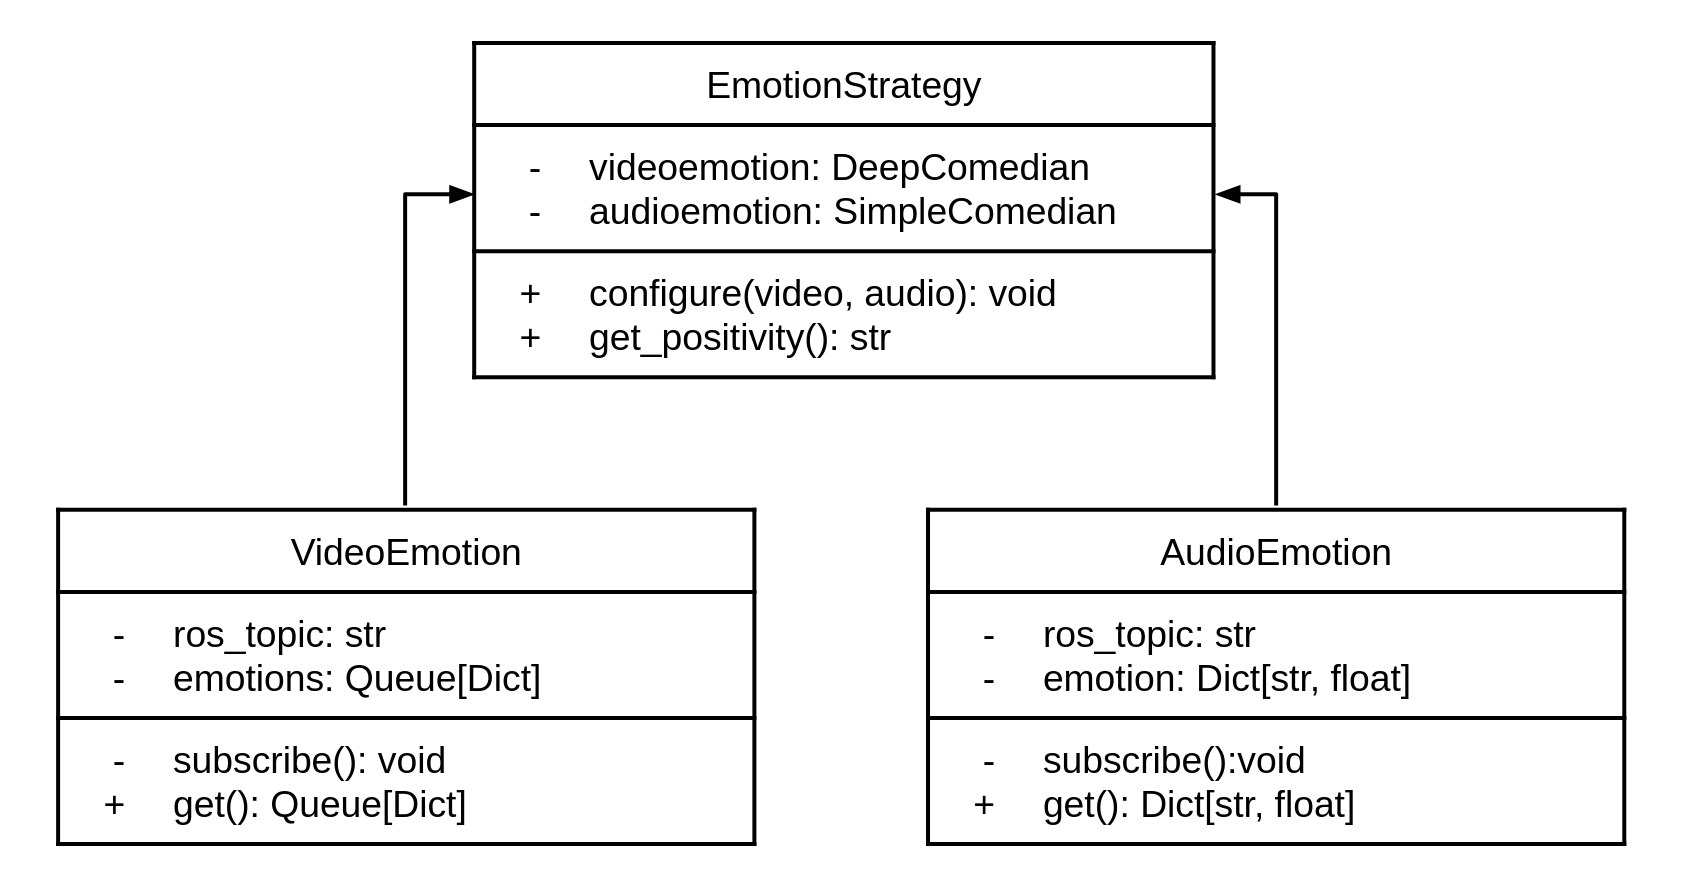
\includegraphics[width=0.8\textwidth]{figures/umlemostr.png}
  \caption{The UML diagram for EmotionStrategy.} \label{fig:umles}
\end{figure}

EmotionStrategy is a class that implements the strategy pattern for the emotion evaluation process (see Figure~\ref{fig:umles}). When initialised, it creates both VideoEmotion and AudioEmotion objects (see Section~\ref{section:ers} in Chapter~\ref{chapter:systemdesign}). The constructor accepts two parameters \( \alpha\) and \( \beta\) which are the weights parameters for \acrshort{fer} and \acrshort{ser} respectively (see Section~\ref{section:ers} in Chapter~\ref{chapter:systemdesign}).

The class features a simple interface that offers two methods:
\begin{itemize}
    \item configure(self, video: bool = True, audio: bool = True) - this method defines the current strategy. There are three available strategies:
    \begin{enumerate}
        \item VideoAudio - when both video and audio parameters are True, this strategy calculates the weighted sum of \acrshort{fer} emotion vectors and \acrshort{ser} emotion vectors
        \item VideoOnly strategy - this strategy chooses only VideoEmotion results and discards AudioEmotion results
        \item AudioOnly - this strategy chooses AudioEmotion results and discards VideoEmotion results
    \end{enumerate}
    \item get\_positivity() -> int, which returns the emotion positivity score as per Section~\ref{subs:V} in Chapter~\ref{chapter:systemdesign}.
\end{itemize}{}

AudioEmotion contains the single Python dictionary [String, Float] field containing seven entries representing a mapping from 7 Rosemo emotions to their emotion recognition scores and a getter method for the data. When EmotionStrategy initialises the AudioEmotion object, the object subscribes to the Rosemo /rosemo\_ser\_pub topic.

VideoEmotion comprises the a custom queue implementation field that contains \( m = f \times w\) dictionaries [String, Float] for each \acrshort{fer} emotion vector containing 7 entries representing a mapping from 7 Rosemo emotions to their emotion recognition scores. It also offers a getter method for the data. When EmotionStrategy initialises VideoEmotion object, the object subscribes to Rosemo /rosemo\_fer\_pub topic.

\section{Rosemo: EmoPy + SER}

\subsection{ROS Interfaces}

Using rospy, we implemented the following ROS topics to communicate from Rosemo to Funboy:
\begin{itemize}
    \item /rosemo\_fer\_pub - the topic for \acrlong{fer} publisher using EmoPy
    \item /rosemo\_ser\_pub - the topic for \acrlong{ser} publisher using \acrshort{ser}
\end{itemize}

We also implemented the following ROS message:
\begin{itemize}
    \item string[] labels
    \item float64[] scores
\end{itemize}
where the string array contains labels of the recognised emotions, and the float array contains emotion recognition scores for each label.

\subsection{Rosemo}

Rosemo is capable of recognising seven basic emotions' labels: calm, anger, happiness, surprise, disgust, fear, sadness - both in speech recordings and in facial image data.

The software module consists of two parts. The first one is video.py script that regularly collects image frames from the camera and processes them. First, it crops the face of the user in the frame using OpenCV. Then it converts the frame into the grey-scale colour range also using OpenCV. After the conversion, it passes the image to EmoPy FERModel classifier. The obtained result is published via ROS to /rosemo\_fer\_pub topic.

The second module is speech.py. When it detects that the user is talking, it records their speech in wave 8 bit, 16kHz format. Then it passes the recording to the \acrshort{ser} CNN-LSTM model. The obtained result is published via ROS to /rosemo\_ser\_pub topic.

\section{Interlocutor Profiles}

To adapt the interlocutors' data for the DARVAH humour affinity scores, we needed to make minor changes to the Ravestate ontology. Therefore, we used the default ontology and made two changes. Firstly, we added new AFFINITY relationship to !OType Person, which is the type used for interlocutors and other known people. Then, we added a new !OType - JokeType:
\begin{itemize}
    \item entity: JokeType
    \item properties: [name, timestamp]
    \item relationships: [EQUALS]
\end{itemize}

\section{Speech Processing}

In the Ravestate Funboy implementation, we based our speech processing capabilities on Roboy Soncreo and roboy\_speech\_recognition software. Both of these packages are own Roboy distributions developed by us utilising pyAudio library for sound processing capabilities. In this project, we used the versions based on Google Cloud Text-to-Speech and Cloud Speech-to-Text services. These modules are accessible from Ravestate via ROS using the following interfaces.

ROS topic for roboy\_speech\_recognition which captures the speech via the microphone stream and publishes a string of text recognised from the stream:
\begin{itemize}
    \item /roboy/cognition/speech/recognition
    \item message type: RecognizedSpeech
    \begin{itemize}
        \item int16 source
        \item string text
        \item float64 start\_timestamp
    \end{itemize}
\end{itemize}
ROS service for Roboy Soncreo - creates and plays a wave file from a passed string of text:
\begin{itemize}
    \item /roboy/cognition/speech/synthesis/talk
    \item service type: Talk
    \begin{itemize}
        \item input: string text
        \item output: bool success
    \end{itemize}
\end{itemize}